\documentclass[twocolumn,DIV18]{scrartcl}
\usepackage{amsmath}
\usepackage{graphicx}
\newcommand{\abs}[1]{\lvert #1 \rvert}
\renewcommand{\(}{\left(}
\renewcommand{\)}{\right)}
%\newcommand{\eqref}[1]{(\ref{#1})}
\begin{document}
\title{Equidistant spiral sampling}
\author{Martin Kielhorn}
\maketitle
\section{Introduction}
We want to illuminate different points in the back focal plane of a
micro objective. Its convenient to have a 1D indexing scheme for these
points. Due to the circular symmetry a spiral sampling [1983Ahn] comes
to mind. 

\section{Archimedes Spiral}
An Archimedes spiral in polar coordinates $(r,\theta)$ is defined like
this:
\begin{align}
  r(\theta)=a\,\theta.
\end{align}
The step height $h$ of the spiral is given by
\begin{align}
  h=\abs{r(\theta)-r(\theta+2\pi)}=r(2\pi)=2\pi a.
\end{align}
\section{Equidistance sampling}
We want to start sampling in the center at $r(0)=0$ and sample the arc
length of the spiral with equidistant points. The arc length of an
archimedes spiral is [Weisstein]:
\begin{align} \label{eqn:arclength}
  s(\theta)=\frac{a}{2}\(p\,\theta + \log(p\,\theta)\)\quad\textrm{with}\quad
  p=\sqrt{1+\theta^2}.
\end{align}
The arc length $\Delta s$ between successive points along the spiral
should be equal to the step height $h$. Starting from the central
point $\theta_0=0$ the arc length where to sample the $i-$th point can
be obtained by inverting equation \eqref{eqn:arclength}:
\begin{align}
  \theta_i=\theta(i\,\Delta s).
\end{align}
This inversion can be done efficiently with Newton interation
[Wikipedia]:
\begin{align}
  x_0&=1,\\
  x_{n+1}&=x_n-\frac{f(x)}{f'(x)}.
\end{align}
Here we introduce the function $f(\theta)$ that vanishes at a given arc
length $s$ and its derivative $f'(\theta)$:
\begin{align}
  f(\theta)&=\frac{a}{2}\(p\,\theta+\log(p\,\theta)-s\),\\
  f'(\theta)&=\frac{\partial f(x)}{\partial x}=a p.
\end{align}
\section{Filling the back focal plane}
Given the number $n$ of sampling points and the desired radius of the
back focal plane $R$ the parameter $a$ and the value of $\theta_n$ can
be determined by solving the following non-linear system of equations:
\begin{align}
  r(\theta_n)=R, \quad \Delta s=2\pi a.
\end{align}
\begin{figure}
  \begin{center}
    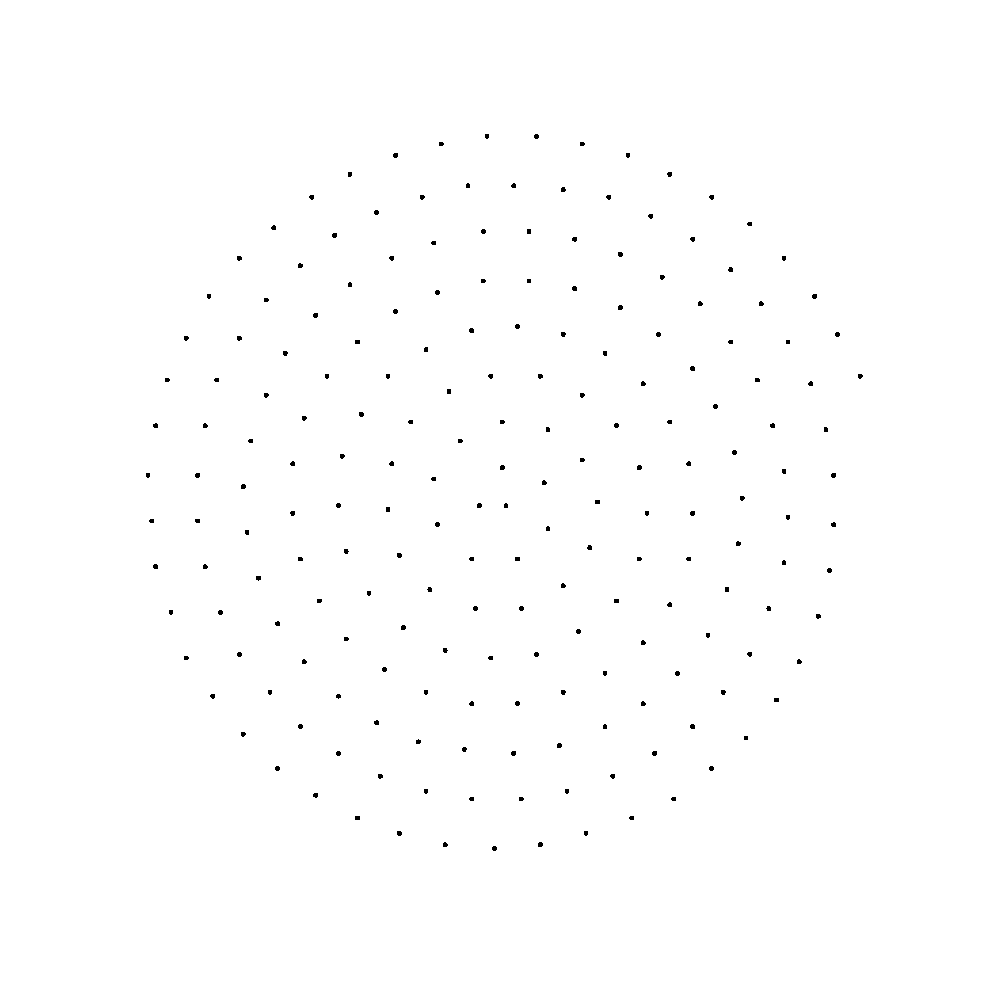
\includegraphics[width=.3\columnwidth]{200}
    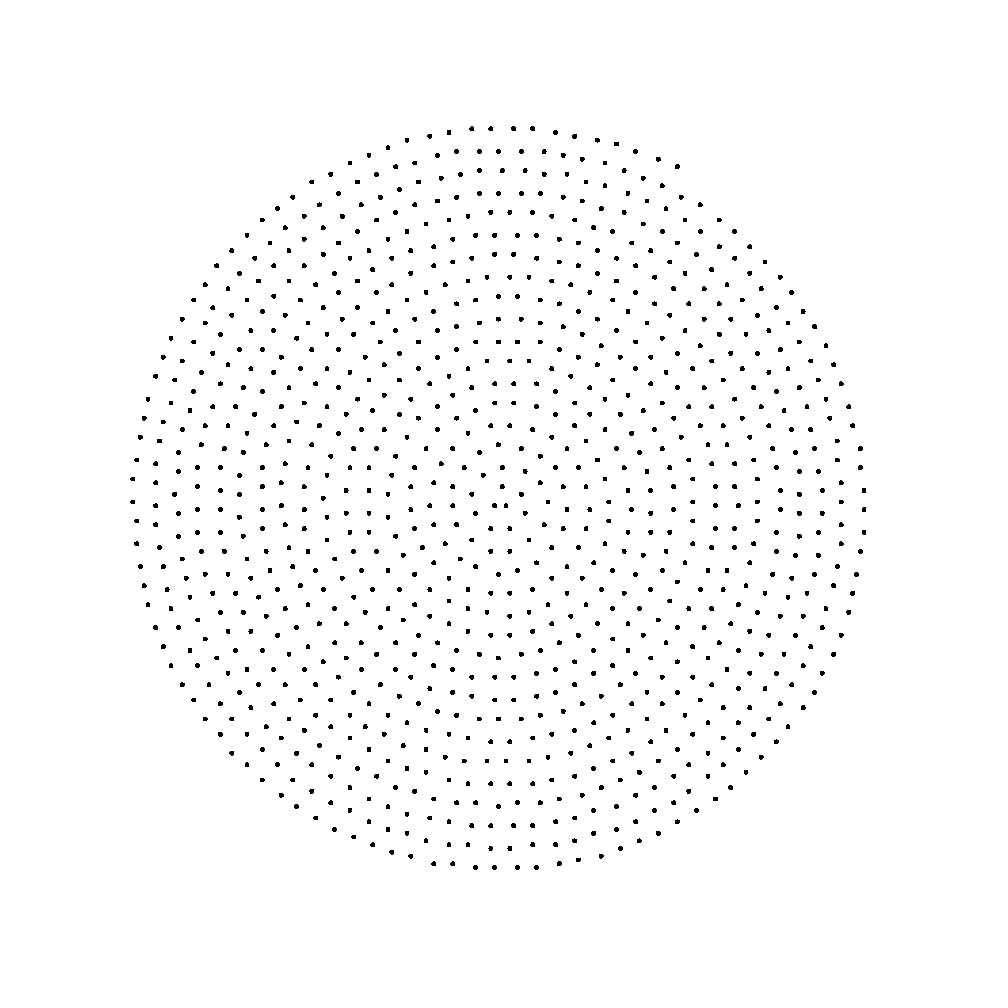
\includegraphics[width=.3\columnwidth]{1000}
    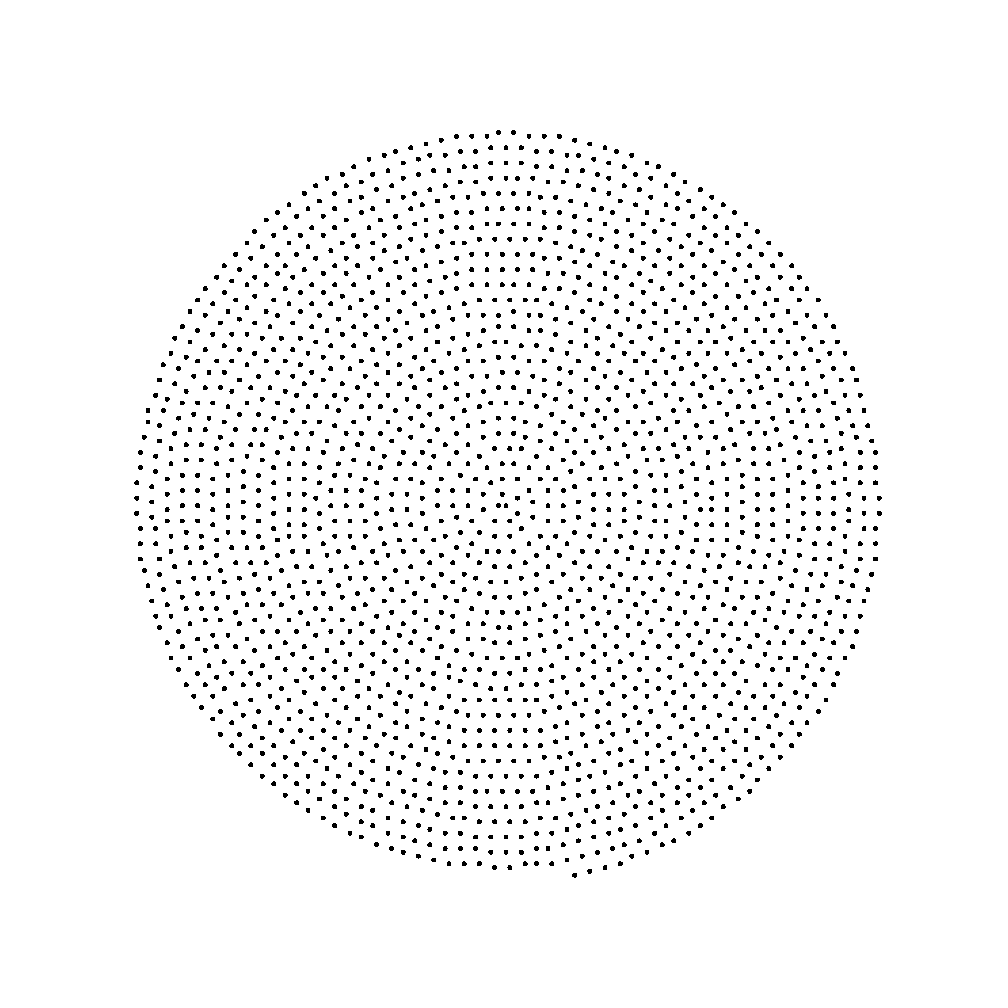
\includegraphics[width=.3\columnwidth]{2000}
  \end{center}
  \caption{Equidistant sampling of a circle of the same diameter with
    200 (left), 1000 (middle) and 2000 (right) points.}
\end{figure}
\end{document}
%% FindRoot[{a x == R, a/2 (Sqrt[1+x^2]x+Log[Sqrt[1+x^2]x]) == n * 2 pi a + R/a}, {{x, 1}, {a, 1}}]

%% @ARTICLE{4307732,
%% author={Ahn, C. B. and Kim, J. H. and Cho, Z. H.},
%% journal={Medical Imaging, IEEE Transactions on}, title={High-Speed Spiral-Scan Echo Planar NMR Imaging-I},
%% year={1986},
%% month={mar.},
%% volume={5},
%% number={1},
%% pages={2 -7},
%% keywords={},
%% doi={10.1109/TMI.1986.4307732},
%% ISSN={0278-0062},}


%% Weisstein, Eric W. "Fibonacci Numbers." From MathWorld--A Wolfram Web Resource. http://mathworld.wolfram.com/FibonacciNumber.html


%% http://en.wikipedia.org/wiki/Newton's_method
